

\section{Synth\`{e}se des connaissances}
Dans cette partie, je d\'{e}taille l'ensemble des connaissances que j'ai accumul\'{e} sur l'impl\'{e}mentation d'un test automatique d'une fonctionnalit\'{e} de Web Intelligence.\\

\subsection{Tests statiques ou dynamiques}

Le test, qu'il soit statique ou dynamique, sera ex\'{e}cut\'{e} avec tous les autres d\`{e}s lors que le nom du test plan est inscrit dans la \gls{Testsuite}\index{Testsuite}.\\
La diff\'{e}rence fonctionnelle entre ces deux types de tests est que l'un ne fait que comparer deux documents Web Intelligence alors que l'autre permet d'appliquer un certain nombre de modifications sans pour autant les comparer syst\'{e}matiquement \`{a} la fin.\\
La diff\'{e}rence en terme de consommation de temps est tr\`{e}s importante, puisque pour un test statique il n'est pas n\'{e}cessaire d'\'{e}crire le code du \gls{Testcase}\index{Testcase}. 

\subsubsection{Tests statiques}
Globalement, le test statique :

\begin{itemize}
	\item compare un document par rapport \`{a} une r\'{e}f\'{e}rence
	\item demande peu de connaissances techniques, que ce soit en \gls{Java} ou sur Web Intelligence
\end{itemize}

La question \`{a} se poser est : \textquote{Quand impl\'{e}menter un test statique?}.\\
Je n'en ai impl\'{e}menté que quelques-uns, l'int\'{e}r\^{e}t en terme de difficult\'{e} et de choses \`{a} apprendre, \'{e}tant limit\'{e}. Mais je pense pouvoir dire qu'un test de ce type n'est utilis\'{e} que pour valider que l'ouverture d'un document se fait correctement. Autrement dit, ce test permet de s'assurer des compatibilit\'{e}s ascendantes de Web Intelligence.\\

\textbf{Principe du test statique}\hfill \\ \indent
Lors de l'ex\'{e}cution d'un test statique, un fichier est g\'{e}n\'{e}r\'{e} \`{a} partir d'un fichier puis, celui-ci est compar\'{e} avec un fichier de r\'{e}f\'{e}rence.\\
Si les deux fichiers sont identiques, le test est correct, sinon il \'{e}choue.\\
Au fur et \`{a} mesure de mes tests j'ai pu d\'{e}duire ce que devait contenir n\'{e}cessairement les diff\'{e}rents fichiers \`{a} impl\'{e}menter et les relations qu'ils entretenaient entre eux.\\
Pour l'ex\'{e}cution d'un test statique, il faut impl\'{e}menter un \gls{Testplan} qui respecte la structure suivante :

\lstinputlisting[language=java]{scripts/basicStaticTest.java}

La premi\`{e}re fois que j'ai compilé un test de ce type, j'ai \'{e}t\'{e} \'{e}tonn\'{e} de le voir \'{e}chouer. Ce que j'ai rapidement compris car son r\^{o}le est de comparer le fichier r\'{e}sultant de ce test avec une r\'{e}f\'{e}rence, r\'{e}f\'{e}rence qui n'existe pas. Le probl\`{e}me auquel j'ai \'{e}t\'{e} confront\'{e} \'{e}tait de savoir comment g\'{e}n\'{e}rer cette r\'{e}f\'{e}rence. J'avais d\'{e}j\`{a} remarqu\'{e} que, gr\^{a}ce \`{a} une configuration particuli\`{e}re du fichier script.xml (voir figure \ref{figure:scriptXmlSavingRef} page \pageref{figure:scriptXmlSavingRef}), des fichiers \'{e}taient g\'{e}n\'{e}r\'{e}s lors de l'ex\'{e}cution de mes tests. Je me suis alors rendu dans le r\'{e}pertoire o\`{u} ces fichiers se trouvaient et ai copié celui-ci dans le dossier des r\'{e}f\'{e}rences. Ceci fait le test n'\'{e}chouait plus, mais comment savoir si ce fichier de r\'{e}f\'{e}rence est fiable? Le r\^{o}le du \gls{Software tester} est de s'assurer que ce fichier peut-\^{e}tre utlis\'{e} comme r\'{e}f\'{e}rence.\\

\begin{figure}[!ht]
  \centering
      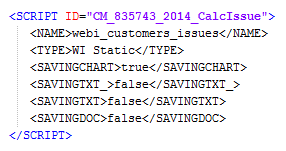
\includegraphics{images/scriptXmlSavingRef.png}
  \caption{Contenu du script.xml pour g\'{e}n\'{e}rer une r\'{e}f\'{e}rence}
	\label{figure:scriptXmlSavingRef}
\end{figure}



\subsubsection{Tests dynamiques}

\`{A} la diff\'{e}rence du test statique, le test dynamique va permettre de modifier le document apr\`{e}s ouverture. Ceci permettant de s'assurer que la m\'{e}canique interne de Web Intelligence produit l'effet escompt\'{e} sur le document.\\
C'est principalement ce type de test que j'ai impl\'{e}ment\'{e}. La grande difficult\'{e} est que, pour chaque test, la logique du code qui doit \^{e}tre impl\'{e}ment\'{e} est compl\`{e}tement diff\'{e}rente. Et surtout il y a toujours plusieurs mani\`{e}res de r\'{e}soudre le probl\`{e}me.\\
J'ai rencontr\'{e} beaucoup de probl\`{e}mes \`{a} impl\'{e}menter ces tests automatiques, pour la simple raison que chacune des fonctionnalit\'{e}s que je devais tester \'{e}tait nouvelle pour moi. Mais en plus de conna\^{i}tre la fonctionnalit\'{e}, ceci se faisant en l'essayant sur une version du produit o\`{u} celle-ci a \'{e}t\'{e} impl\'{e}ment\'{e}e, il faut pouvoir en reproduire le fonctionnement au niveau SDK.\\
\`{A} cette fin, le plus pratique \'{e}tait d'aller voir directment dans le code du produit ce qu'il se passait. Mais ce n'\'{e}tait pas toujours facile et j'ai pass\'{e} beaucoup de temps \`{a} investiguer pour parfois ne rien trouver.\\
La m\'{e}thode que j'utilisais \'{e}tait de me connecter au client DHTML de Web Intelligence, de cette mani\`{e}re je pouvais utiliser le d\'{e}bugger du navigateur, et ceci me permettait deux choses :
\begin{enumerate}
	\item observer les donn\'{e}es qui transitaient et les quelques variables et m\'{e}thodes en jeu. De l\`{a}, je pouvais conna\^{i}tre les classes concern\'{e}es par la fonctionnalit\'{e} \`{a} tester. Cette \'{e}tape est particuli\`{e}rement p\'{e}nible et porte rarement ses fruits. J'ai d'abord eu de grandes difficult\'{e}s \`{a} d\'{e}celer les bonnes donn\'{e}es dans le flot continu d'information. Les quelques fois o\`{u} j'arrivais \`{a} trouver une information (une m\'{e}thode dont le nom laisse entendre qu'elle a quelque chose \`{a} voir avec ce que je cherche), il me fallait retrouver l'impl\'{e}mentation concern\'{e}e dans le code du produit, \'{e}tape rendue tr\`{e}s difficile par la tr\`{e}s grande quantit\'{e} de classes et d'\gls{Interface}s diff\'{e}rentes.
	\item ex\'{e}cuter le \gls{Workflow} pour arriver jusqu'au bug pour d\'{e}celer la portion du code o\`{u} l'anomalie survient. Les difficult\'{e}s rencontr\'{e}es sont les m\^{e}mes que pour le point pr\'{e}c\'{e}dent.
\end{enumerate}


Outre le fait de trouver le moyen de tester la fonctionnalit\'{e}, j'ai rencontr\'{e} un certain nombre de probl\`{e}mes \`{a} impl\'{e}menter le test automatique, car il en existe de toute sorte et son impl\'{e}mentation de base n'\'{e}tait pas la m\^{e}me en fonction de ce que je voulais faire avec. Au fur et \`{a} mesure de mon exp\'{e}rience, je me suis construit une impl\'{e}mentation g\'{e}n\'{e}rique qui permettait de me faire gagner un temps pr\'{e}cieux. Les codes que je me suis ainsi construit (\gls{Testplan} et \gls{Testcase}) et que je copiais/collais sont les suivants :

\lstinputlisting[language=java,label=basicDynamicTestPlan]{scripts/basicDynamicTestPlan.java}


Et son testcase respecte l'impl\'{e}mentation suivante :

\lstinputlisting[language=java,label=basicDynamicTestCase]{scripts/basicDynamicTestCase.java}



%\begin{figure}[H]
  %\centering
      %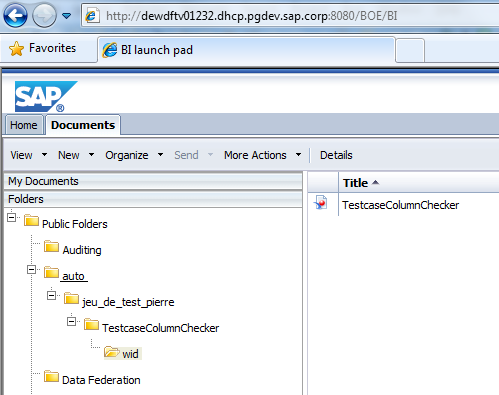
\includegraphics{images/savedReferenceDocPath.png}
  %\caption{Capture d'\'{e}cran de WebI de l'arborescence du document de r\'{e}f\'{e}rence}
	%\label{figure:savedReferenceDocPath}
%\end{figure}
%\begin{figure}[H]
  %\centering
      %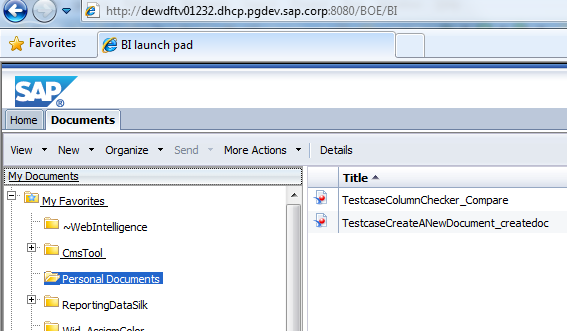
\includegraphics{images/savedGeneratedDocPath.png}
  %\caption{Capture d'\'{e}cran de WebI de l'arborescence du document g\'{e}n\'{e}r\'{e}}
	%\label{figure:savedGeneratedDocPath}
%\end{figure}


\subsection{De l'\'{e}tude \`{a} l'int\'{e}gration}

D'abord, les demandes de tests automatiques ne sont pas toujours r\'{e}alisables au niveau SDK. Il convient donc de v\'{e}rifier, en premier lieu, la faisabilit\'{e} du test. Cette \'{e}tape n\'{e}cessite de particuli\`{e}rement bien conna\^{i}tre le produit pour savoir si telle ou telle action est effectu\'{e}e au niveau \gls{SDK}. La m\'{e}thode que j'utilisais \'{e}tait de tester la fonctionnalit\'{e} sur le client DHTML afin de savoir quelles m\'{e}thodes \'{e}taient appel\'{e}es. Ensuite, je me rendais dans le code de Web Intelligence afin de rechercher le code en question. Si les appels en question se faisaient du SDK, je pouvais impl\'{e}menter mon test, sinon, si les appels \`{a} tester se faisaient plus bas dans l'architecture, je ne pouvais pas impl\'{e}menter le test.\\
Cette mani\`{e}re de proc\'{e}der est longue et sa complexit\'{e} ne me garantissait pas d'arriver \`{a} mes fins. De sorte qu'en r\`{e}gle g\'{e}n\'{e}rale je n'arrivais pas \`{a} trouver la r\'{e}ponse. J'essayais toujours mais je finissais souvent par impl\'{e}menter le test sans savoir si cela serait possible d'en arriver au terme. Cela m'a valu de perdre beaucoup de temps \`{a} impl\'{e}menter des codes qui, au final, n'ont jamais servi.\\

Pour analyser le test automatique \`{a} impl\'{e}menter je devais d'abord essayer le \gls{Workflow} qui faisait survenir l'anomalie sur Web Intelligence. Toutes les informations que l'on a sur celle-ci se trouvent sur JCWB\index{\gls{Java} Correction WorkBench} (voir figure \ref{figure:JCWB-CRs} page \pageref{figure:JCWB-CRs}) ou Jira\index{Jira}, je pouvais alors conna\^{i}tre :
\begin{itemize}
	\item L'identifiant du defect (utilis\'{e} par les conventions de nommage)
	\item La description d\'{e}taill\'{e}e du \gls{Workflow} pour faire l'exp\'{e}rience de l'anomalie
	\item La/Les branche(s) sur laquelle/lesquelles elle a \'{e}t\'{e} d\'{e}cel\'{e}e, de mani\`{e}re \`{a} en faire l'exp\'{e}rience deux fois. La premi\`{e}re pour v\'{e}rifier l'existence de l'anomalie et la seconde pour valider que celle-ci a \'{e}t\'{e} correctement corrig\'{e}e.
\end{itemize}
\begin{figure}[!ht]
  \centering
      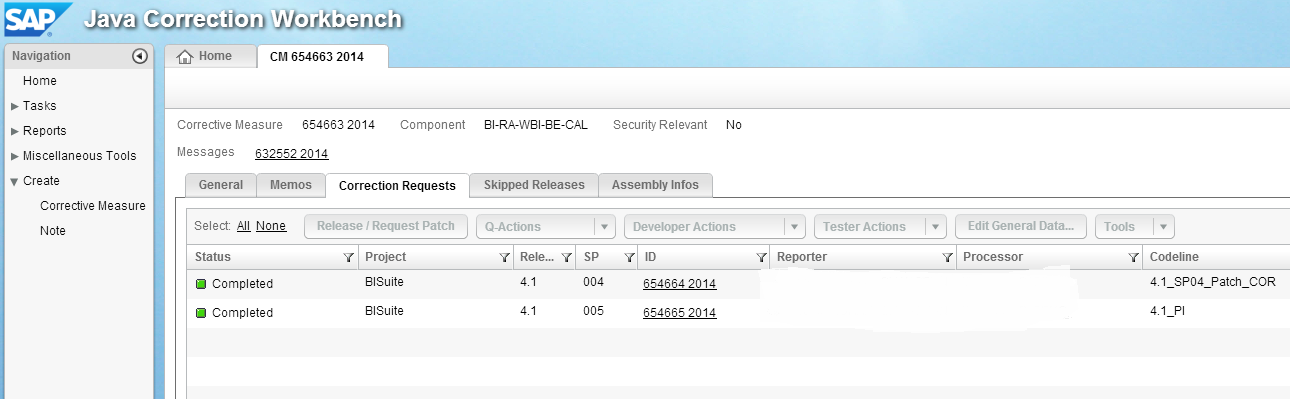
\includegraphics[width=\textwidth]{images/JCWB-CRs.png}
  \caption{\'{E}cran de JCWB propre \`{a} une CM\index{Correction Measure}}
	\label{figure:JCWB-CRs}
\end{figure}

Cette partie pr\'{e}alable \`{a} l'impl\'{e}mentation du test automatique m'a permis de manipuler le produit Web Intelligence et plus particuli\`{e}rement les fonctionnalit\'{e}s que je devais tester. J'ai appris beaucoup de choses sur son utilisation et ses fonctionnalit\'{e}s. \\
Pour cela j'ai du apprendre \`{a} l'utiliser, cr\'{e}er des rapports et effectuer des changements dessus. Web Intelligence est un produit incroyablement riche en fonctionnalit\'{e}s dans lequel il est possible de faire beaucoup de choses. Cette exp\'{e}rience est d'autant plus riche que toutes les connaissances et savoir-faire que j'ai acquis pourront me servir dans le futur. Je suis tr\`{e}s loin de ma\^{i}triser Web Intelligence mais j'ai pu en comprendre l'utilit\'{e} et la logique d'utilisation. Je serai donc capable, \`{a} l'avenir, de faire valoir cette comp\'{e}tence.\\

Lors de mes investigations sur les fonctionnalit\'{e}s et les anomalies, en plus de devoir reproduire le \gls{Workflow} \`{a} la main depuis l'interface graphique, je devais \'{e}tudier les correctifs appliqu\'{e}s pour orienter ma logique d'impl\'{e}mentation du \gls{Testcase}. Cela a \'{e}t\'{e} tr\`{e}s formateur car les diff\'{e}rents codes que j'\'{e}tudiais avaient \'{e}t\'{e} impl\'{e}mentés par des d\'{e}veloppeurs confirm\'{e}s. Il est connu que c'est en lisant le code d'autrui que l'on progresse, et j'ai appris \'{e}norm\'{e}ment de choses, tant du point de vue de la logique de la programmation orient\'{e}e objet que de la complexit\'{e} des proc\'{e}dures utilis\'{e}es. De plus, en observant les modifications faites pour corriger l'anomalie j'ai pu comprendre plus en d\'{e}tail les diff\'{e}rentes raisons qui font qu'une telle anomalie puisse exister (voir l'interface graphique qui me permettait de faire ces observations figure \ref{figure:diffAgainst} page \pageref{figure:diffAgainst}). Ce qui peut \^{e}tre, entre autre, une condition manquante, un probl\`{e}me d'identifiant ou une m\'{e}moire satur\'{e}e.\\


\begin{figure}[!ht]
  \centering
      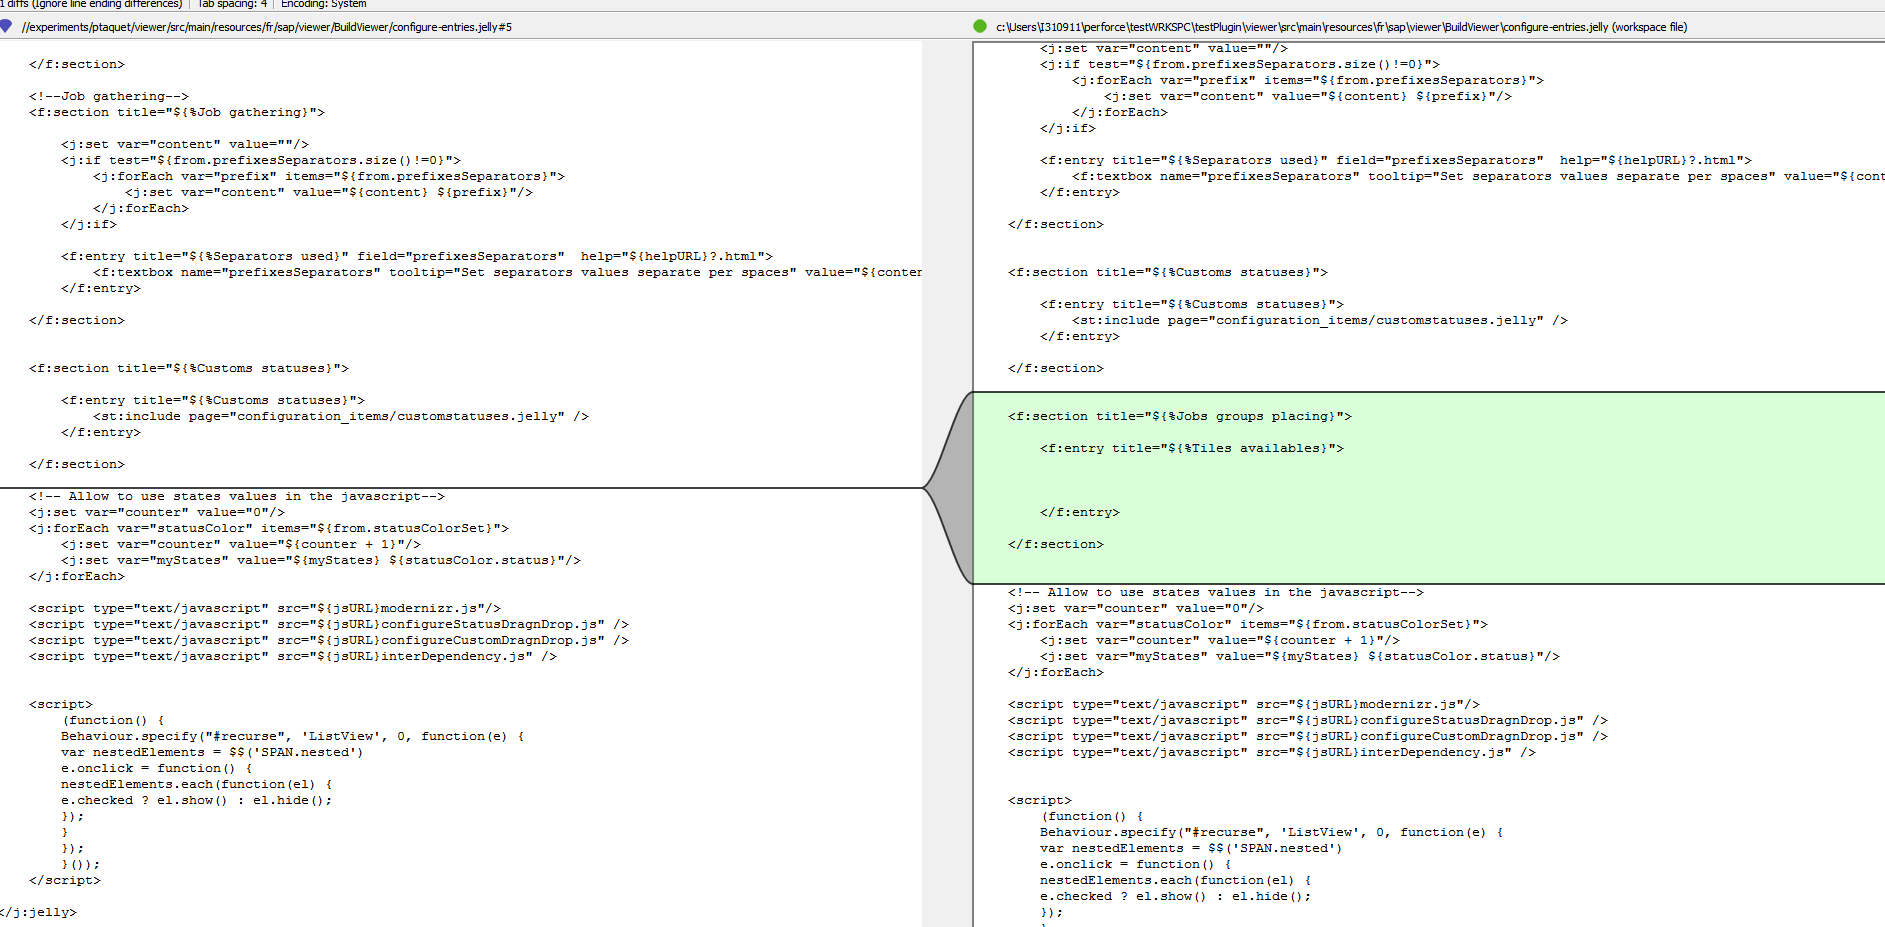
\includegraphics[width=\textwidth]{images/diffAgainst.png}
  \caption{\'{E}cran de comparaison des 2 versions d'un m\^{e}me fichier (avant et apr\`{e}s correctif)}
	\label{figure:diffAgainst}
\end{figure}




\subsubsection{Impl\'{e}mentation de la coquille vide}

Apr\`{e}s avoir fait l'\'{e}tude de l'anomalie, il faut commencer \`{a} impl\'{e}menter le test automatique. La premi\`{e}re difficult\'{e} que j'ai rencontr\'{e} \'{e}tant le choix du point de d\'{e}part, il en existe plusieurs. Mon tuteur m'a guid\'{e} dans le choix de ceux-ci et m'en a expliqu\'{e} les diff\'{e}rents int\'{e}r\^{e}ts. Il \'{e}tait difficile de comprendre comment et pourquoi utiliser l'un ou l'autre car cela d\'{e}pendait directement de ce qui devait \^{e}tre fait dans le test automatique. Si le test portait sur des \'{e}l\'{e}ments graphiques ou des configurations il \'{e}tait plus simple de baser son test sur un document Web Intelligence, car celui-ci me permettait d'appliquer la majeure partie des actions accessibles depuis l'interface graphique. Si je voulais plut\^{o}t v\'{e}rifier un contenu quelconque, il \'{e}tait plus simple de se baser sur une \gls{Queryspec} car toutes les donn\'{e}es y sont directement accessibles. \\

J'ai majoritairement utilis\'{e} les documents Web Intelligence pour d\'{e}marrer mes tests. Mais, une fois, je me suis retrouv\'{e} confront\'{e} \`{a} un probl\`{e}me que je ne pouvais pas r\'{e}soudre car je n'avais pas choisi la queryspec. Je voulais acc\'{e}der \`{a} une information du document qui n'\'{e}tait pas disponible depuis le \gls{SDK}, en utilisant le document Web Intelligence, mais qui l'\'{e}tait depuis la queryspec. J'ai cherch\'{e} pendant de longues heures, en \'{e}tant au plus proche de ce que je cherchais mais malheureusement aux limites de ce que le \gls{SDK} me permettait de faire. Je n'ai jamais r\'{e}ussi \`{a} r\'{e}soudre le probl\`{e}me seul, je suis donc all\'{e} voir mon tuteur pour exposer mon probl\`{e}me, celui-ci m'a expliqu\'{e} le pourquoi de l'obstacle que je rencontrais et m'a conseill\'{e} d'utiliser plut\^{o}t la queryspec. Apr\`{e}s \^{e}tre retourn\'{e} dans mon bureau, j'ai pu r\'{e}soudre mon probl\`{e}me et finir d'impl\'{e}menter mon test automatique avant la fin de la journ\'{e}e.\\

Plus que d'avoir heurt\'{e} les limites du champ d'action du \gls{SDK}, ma principale erreur a \'{e}t\'{e} de ne pas me diriger plus t\^{o}t vers la personne qui aurait pu me conseiller, cela m'aurait \'{e}pargn\'{e} plusieurs heures d'efforts inutiles.\\

Le choix du point de d\'{e}part pour impl\'{e}menter un test automatique est donc tr\`{e}s important. Mais quelque soit ce choix, il faut aussi impl\'{e}menter la coquille vide de ce test, qui est, dans tous les cas, quasiment similaire. La coquille vide permet d'avoir un code qui compile mais qui ne fait encore rien. Ce qui garantit que tous les \'{e}l\'{e}ments sont bien reli\'{e}s entre eux. Car, comme sch\'{e}matis\'{e} figure \ref{figure:testsRelations} page \pageref{figure:testsRelations}, chaque test automatique est int\'{e}gr\'{e} \`{a} un \gls{Testplan}, lui-m\^{e}me int\'{e}gr\'{e} \`{a} une \gls{Testsuite}.\\
\begin{figure}[!ht]
  \centering
      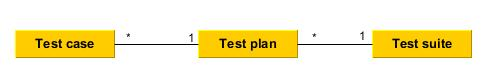
\includegraphics[width=\textwidth]{images/testsRelations.jpg}
  \caption{Diagramme UML des suites de tests}
	\label{figure:testsRelations}
\end{figure}

Les fichiers essentiels au bon fonctionnement du test sont d\'{e}crits ci-dessous. Il n'\'{e}tait pas \'{e}vident, au d\'{e}but, de compl\'{e}ter correctement tous ces documents car chacun a une utilit\'{e} tr\`{e}s particuli\`{e}re :
\begin{itemize}
	\item Test plan
	\item Test case
	\item Test suite
	\item script.xml
	\item ressources (\gls{Queryspec}\index{queryspec} ou document Web Intelligence)
	\item parameters.xml
\end{itemize}

La principale difficult\'{e} que j'ai rencontr\'{e} lors de l'impl\'{e}mentation de la coquille a \'{e}t\'{e} la convention de nommage. En effet, la moindre erreur ne permet pas au test de compiler.\\
Pour illustrer la coquille vide du test automatique et pour permettre de les visualiser dans la structure du \gls{Framework}, je les ai repr\'{e}sent\'{e} dans la figure \ref{figure:testEmptyShell} page \pageref{figure:testEmptyShell}. Et, de la m\^{e}me mani\`{e}re, la figure \ref{figure:usedFilesForTests} page \pageref{figure:usedFilesForTests} pr\'{e}sente le test avec les diff\'{e}rents documents avec lesquels celui-ci interagit.\\
Les ressources sont tr\`{e}s importantes dans le contexte du test, et j'ai eu quelques difficult\'{e}s au d\'{e}but pour arriver \`{a} les g\'{e}n\'{e}rer rapidement.\\
Il m'est arrivé plusieurs fois de g\'{e}n\'{e}rer des fichiers de r\'{e}f\'{e}rences \`{a} partir de la mauvaise version, ce qui avait pour effet de faire \'{e}chouer mes tests sans que je puisse, rapidement, savoir pourquoi.\\
\begin{figure}[H]
  \centering
      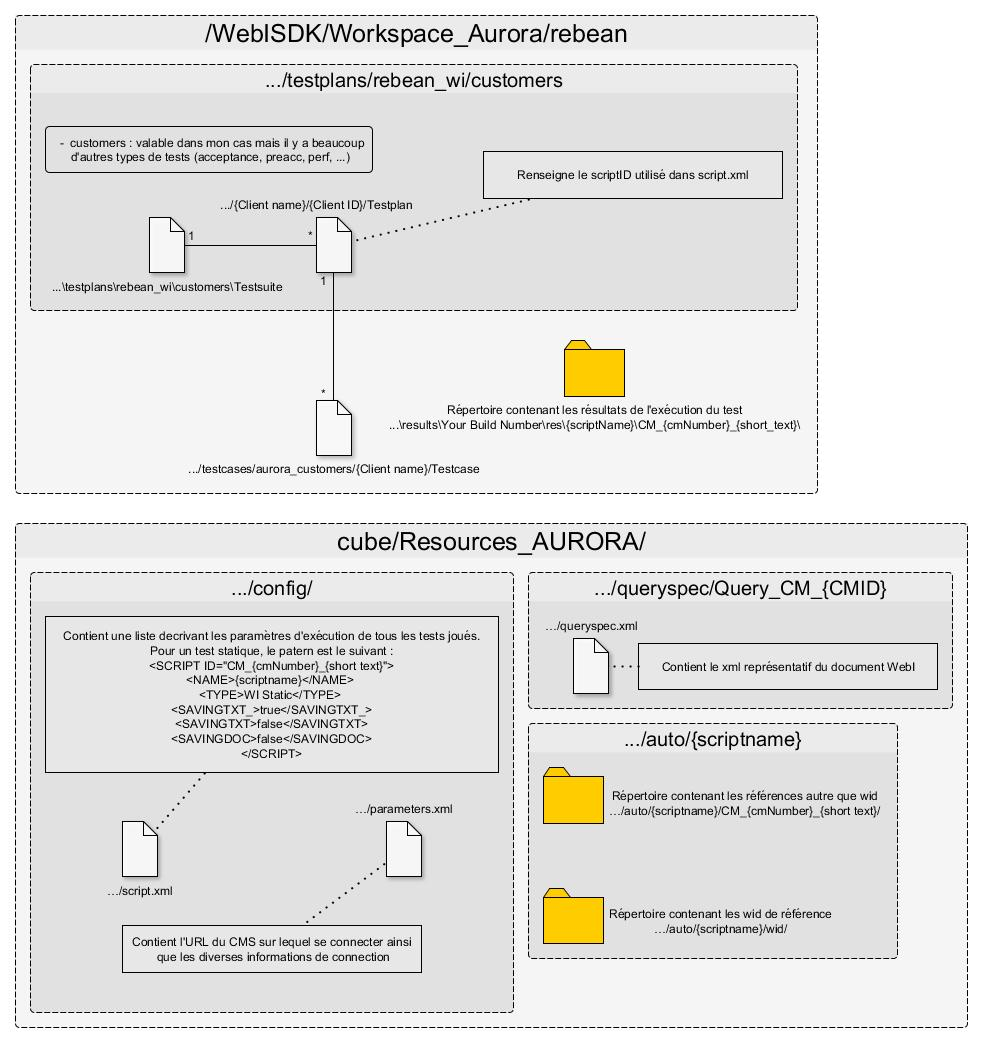
\includegraphics[width=\textwidth]{images/testEmptyShell.jpg}
  \caption{Diagramme repr\'{e}sentant les diff\'{e}rents \'{e}l\'{e}ments qui compose la coquille vide d'un test dynamique}
	\label{figure:testEmptyShell}
\end{figure}
\begin{figure}[H]
  \centering
      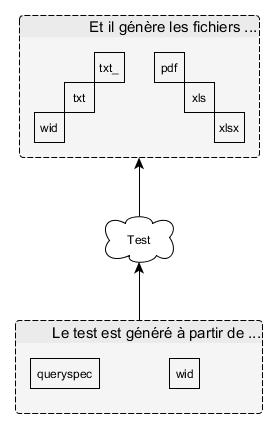
\includegraphics[width=0.4\textwidth]{images/usedFilesForTests.jpg}
  \caption{Les fichiers utilis\'{e}s ou g\'{e}n\'{e}r\'{e}s par le test}
	\label{figure:usedFilesForTests}
\end{figure}

\subsubsection{Les ressources}

Comme j'en ai d\'{e}j\`{a} parl\'{e} plus haut, il existe plusieurs types de ressources. Les deux principales \'{e}tant le document Web Intelligence et la \gls{Queryspec}.
Il y a deux mani\`{e}res d'obtenir un document Web Intelligence, les deux sont similaires.\\
\textbf{Obtenir un fichier wid\index{wid}}
\begin{description}
	\item	[Via le CMS\index{CMS}] 
	\begin{sloppypar}
	Il suffit de parcourir l'arborescence du CMS\index{CMS} pour arriver \`{a} l'emplacement du .wid\index{wid}. Dans les propri\'{e}t\'{e}s du fichier, il y a son nom complet (diff\'{e}rent du nom dans WebI) avec son arborescence \`{a} partir du dossier Input (figure \ref{figure:widFileLocation} page \pageref{figure:widFileLocation} ). Ensuite, dans le syst\`{e}me de fichiers du serveur (par exemple : \textquote{\textbackslash{}\textbackslash{}dewdftv01634.dhcp.pgdev.sap.corp\textbackslash{}c\$}) aller dans 
	\textquote{\textbackslash{}Program Files (x86)\textbackslash{}SAP BusinessObjects\textbackslash{}SAP BusinessObjects Enterprise XI 4.0\textbackslash{}FileStore\textbackslash{}Input} et copier/coller le chemin d'acc\`{e}s au fichier. Le document Web Intelligence se trouve dans le r\'{e}pertoire en question.
	\end{sloppypar}
\begin{figure}[!ht]
  \centering
      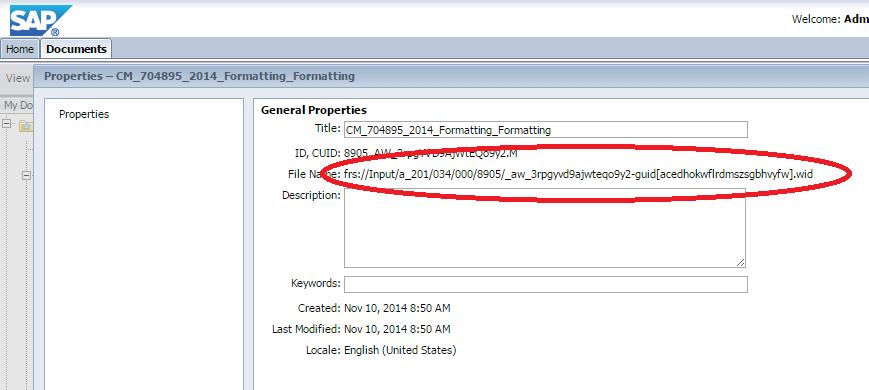
\includegraphics[width=\textwidth]{images/widFileLocation.png}
  \caption{Capture de l'\'{e}cran de propri\'{e}t\'{e} d'un document WebI}
	\label{figure:widFileLocation}
\end{figure}
	\item[Via le Rich Client]
	Avec ce proc\'{e}d\'{e} il faut faire attention \`{a} la version du rich client qui doit \^{e}tre la m\^{e}me que celle du CMS\index{CMS}, une erreur se traduit par un fichier de r\'{e}f\'{e}rence erron\'{e}, donc un test qui \'{e}choue. J'ai fait cette erreur plusieurs fois, au d\'{e}but, car j'avais toujours plusieurs versions de Web Intelligence qui \'{e}taient ouvertes. L'utilisation du \gls{Client lourd} est la plus instinctive car il suffit d'ouvrir le document et de l'enregistrer en local.
\end{description}
